\mySection{10.4  Goodness-of-Fit Tests: Parameters Unknown}
%-------------- start slide -------------------------------%{{{ 10.37
\begin{frame}
	% {\S\: 10.4  Goodness-of-Fit Tests: Parameters Unknown}
\begin{center}
\renewcommand{\arraystretch}{2}
\begin{tabular}{c|c}
	$p_i$ are known \cellcolor{gray!50!background}                  & $p_i$ are unknown \cellcolor{gray!50!background}                           \\ \hline
	$D=\sum_{i=1}^t  \frac{\left(X_i-np_i \right)^2}{np_i}$         & $D_1=\sum_{i=1}^t  \frac{\left(X_i-n\hat p_i \right)^2}{n \hat p_i}$       \\
	$\chi^2$ with f.d. $t-1$                                        & $\chi^2$ with f.d. $t-1-s$                                                 \\
	$d=\sum_{i=1}^t  \frac{\left(k_i-n p_{i0} \right)^2}{n p_{i0}}$ & $d_1=\sum_{i=1}^t  \frac{\left(k_i-n\hat p_{i0} \right)^2}{n \hat p_{i0}}$ \\
	$np_{i0}\ge 5$                                                  & $n\hat p_{i0}\ge 5$                                                        \\
	$d>\chi^2_{1-\alpha,t-1}$                                       & $d_1>\chi^2_{1-\alpha,t-1-s}$
\end{tabular}
\end{center}
\vfill
\begin{enumerate}
\item[$\dagger$] $s$ is the number of unknown parameters.\\
\[
\text{df} = \text{\underline{number of classes}} -1 -
\text{\underline{number of unknown parameters.}}
\]
\end{enumerate}
\end{frame}
%-------------- end slide -------------------------------%}}}
%-------------- start slide -------------------------------%{{{ 10.38
\begin{frame}
\begin{enumerate}
\item[E.g. 1] Binomial data:
4096 students, each shots basketball $4$ times.
Let $X_i$ be the number of hits for the $i$th student.
\begin{center}

\includegraphics[scale=0.1]{MM_twocolors-neg.jpeg}	\qquad
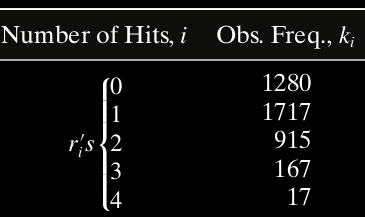
\includegraphics[scale=0.3]{Table_10-4-1-1-neg.png}
\end{center}
\item[] People believe that $X_i$ should following binomial$(4,p)$, that is,
shotting basketball should be something like trying to get red chocolate beans
from a jar of beans of two colors.\\[1em]
\item[] Find the MLE for $p$. Use the data to make a conclusion.
\vfill
\item[Sol.] 1) $H_0:$ $X_i\sim$binomal($4,p$).\\[1em]
\item[] 2) Under $H_0$, the MLE for $p$ is $p_e= ... = 0.251$
\end{enumerate}
\end{frame}
%-------------- end slide -------------------------------%}}}
%-------------- start slide -------------------------------%{{{ 10.39
\begin{frame}

\begin{enumerate}
\item[] 3) Compute the expected frequenies:
\begin{center}
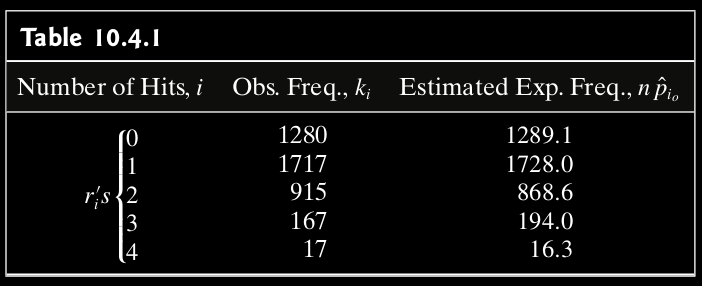
\includegraphics[scale=0.3]{Table_10-4-1-neg.png}
\end{center}
\[
\Longrightarrow\quad			d_1 = \cdots = 6.401.
\]
\vfill
\item[] 4) Critical region: $(\chi^2_{.95,5-1-1},+\infty) =(7.815,+\infty) $
\item[] 5) Conclusion: Fail to reject.
\vfill
\item[] 6) Alternatively, $P$-value $=\bbP(\chi_3^2\ge 6.401) =  0.094$, ... discuss...\myEnd
\end{enumerate}
\end{frame}
%-------------- end slide -------------------------------%}}}
%-------------- start slide -------------------------------%{{{ 10.40
\begin{frame}

\begin{enumerate}
\item[E.g. 2] Does the number of death per day follow the Poisson distribution?
	\vfill
\begin{center}
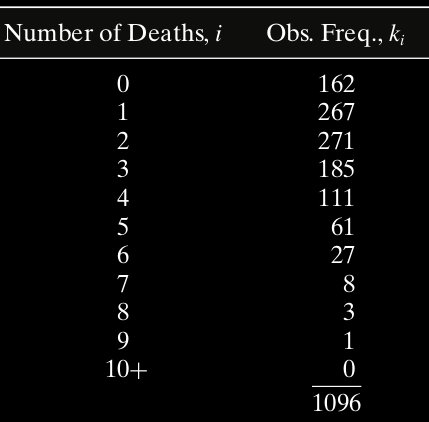
\includegraphics[scale=0.3]{Table_10-4-2-1-neg.png}
\end{center}
\end{enumerate}
\end{frame}
%-------------- end slide -------------------------------%}}}
%-------------- start slide -------------------------------%{{{ 10.41
\begin{frame}
	\begin{enumerate}
		\item[Sol.] 1) Let $X_i$ be the number of death in $i$th day, $1\le i\le 1096$.\\
			\vfill
		\item[] 2) $H_0:$ $X_i$ follow Poisson$(\lambda)$.
			\vfill
		\item[] 3) The MLE for $\lambda$ is: $\lambda_e = \cdots = 2.157$.
			\vfill
		\item[] 4) Compute the expected frequencies:
\begin{center}
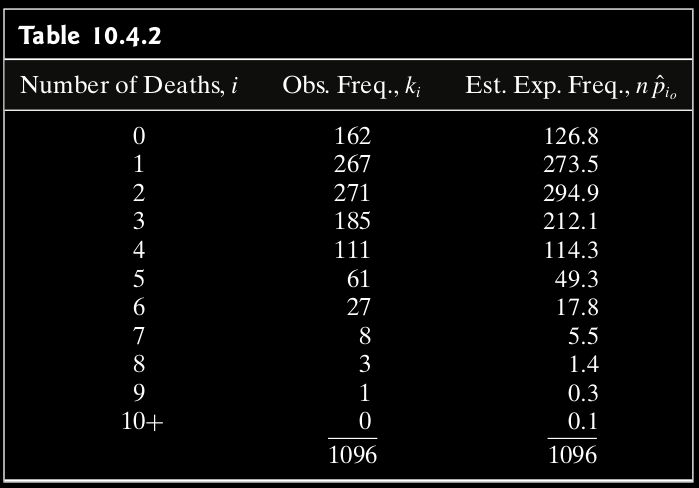
\includegraphics[scale=0.2]{Table_10-4-2-neg.png}
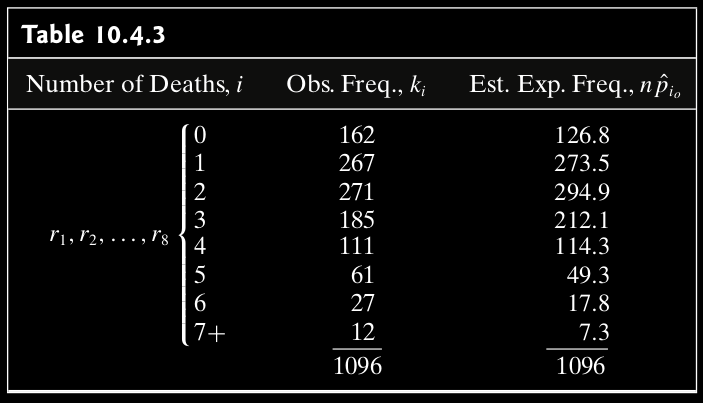
\includegraphics[scale=0.2]{Table_10-4-3-neg.png}
\end{center}
\pause
\[
\Longrightarrow \quad d_1 = \cdots = 25.98.
\]
\vfill
\pause
\item[] 5) $P$-value $= \bbP(\chi_{1,8-1-1}^2\ge 25.98) =0.00022$. Reject! \myEnd
	\end{enumerate}
\end{frame}
%-------------- end slide -------------------------------%}}}
